\section{Proposed ChatBot}
%
\subsection{DataModel}
It seems obvious that browsing our 2,249,053 lines-long corpus for each query wasn't such a great idea, that's why we stored the data in a re-usable DBMS.
\subsubsection{Chosen technology}
We considered 2 options : a traditional DBMS such as MySQL or a graph-oriented DBMS. We finally chose to use a graph model for several reasons :
\begin{itemize}
\item For a corpus such as ours, with a lot of n-1..n relations, a graph allows the user to build queries who look like \say{paths}. It is both more efficient (no table join, less computation time) and more natural for the user.
\item Graph-base DBMS doesn't require a rigid schema, which means that we can create new kind of entities and relationships \say{on the go}.
\item It supports indexes and unique constraints
\item Most of the graph-based systems implements useful algorithms such as the shortest path between two nodes.
\end{itemize}
Regarding the technology, Neo4j\footnote{http://neo4j.com/} was chosen in regards of those facts :\\
\begin{itemize}
\item One of us (Mael) was already working with it for his MasterArbeit and was familiar with the language used to build Neo4j queries (Cypher).
\item Neo4j is cross-platform
\item The community is strong, there're even french groups
\item The technology is mature, 15 years old and currently running version 2.2
\item It provides a nice browser interface
\end{itemize}

\subsubsection{Structure}
Here, we will describe the actual structure of the corpus-graph. Remember that it isn't rigid so it might vary over the project's progress.\\
Other nodes and relationships exist in our database but are used for other purposes such as the history of the conversation or some probabilities (see section \ref{sssec:v_stype}).\\
Basically we can say that in our case, one vertex equals one XML tag. Instead of listing all the vertexes and the edges, we provide here an example based on a dialogue from the movie\footnote{12 Monkeys on IMDB : http://www.imdb.com/title/tt0114746/} \say{12 Monkeys}.
\lstinputlisting[language=XML,caption=XML extract,label={code:extr}]{./prim/graphExample.xml}
\begin{figure}[!h]
\begin{center}
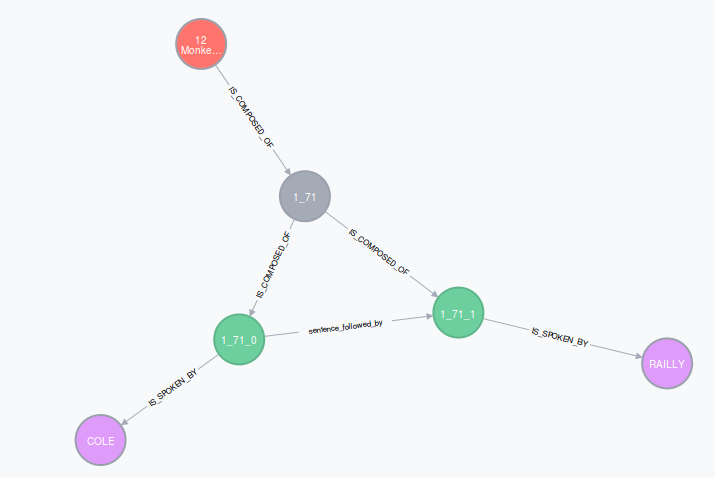
\includegraphics[width=0.8\textwidth]{./img/graph171.png}
\end{center}
\caption{Neo4j modelisation}
\label{fig:neoExtr}
\end{figure}
With the above example we see that, just like in the XML (Code \ref{code:extr}), a \textbf{Movie} (pink) \textit{IS\_COMPOSED\_OF} \textbf{Dialogues} (gray, only one displayed here) which \textit{IS\_COMPOSED\_OF} several \textbf{Sentences} (green). Each sentence \textit{IS\_SPOKEN\_BY} a \textbf{Character} (purple).\\
We store the full sentence as an attribute of the Sentence node. The labels of the dialogues and sentences are an aggregation of the id fields of their parents :
\begin{center}Sentence\_Node\_id = idMovie\_idDialogue\_idSentence \end{center}
Now that we have represented the corpus as a graph, we can start to work with the NLP technology. Each sentence his processed and \dots \\
\textbf{LEO, BLABLA A PROPOS DU DECOUPAGE EN TOKEN ET LES SENTENCESTYPES, REF A FIG.15}
\begin{figure}[!h]
\begin{center}
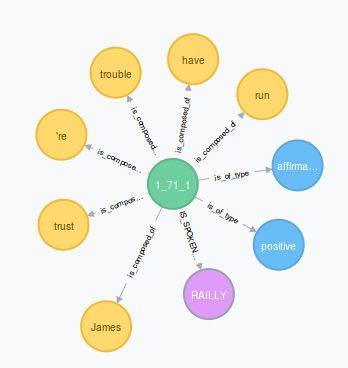
\includegraphics[width=0.5\textwidth]{./img/graph1711.png}
\end{center}
\caption{Sentence details}
\label{fig:sent}
\end{figure}

%
\subsection{User Interface}
\subsubsection{Chosen technology}
\label{subs:Technology}

\paragraph{State of the Art}
\label{par:SotA}
Obviously, this is a Python project, because the point of the course is to discover NLP and Text-mining by using NLTK.
So, we decided to naturally go and try our way in Python to get an interface for our chat-bot.
In the litterature, there are two main approaches for doing that :
\begin{itemize}
    \item Interfacing our bot on an IRC server, and using an IRC client as a User Interface.
    \item Developing our own interface.
\end{itemize}
As we wanted the user to be able to rate our bot's answers, the first solution was never really an option.
An IRC (or so) client's interface doesn't give us room for non-textual interaction, and it is something which was important for us.
The second solution, developing our own interface, is quite easy in Python, as long as you have more than just notions in web development.
We explored two Python frameworks, \textit{Django} and \textit{Flask}.
\textit{Django} is obviously way too dense and heavy for our needs, so we tried our best with Flask.
Considering that the user interface is not a very important component of our application, we decided that Flask was also a waste of time for us, and that we should do what we could already do.

\paragraph{Shiny}
\label{par:Shiny}
Therefore we decided to propose a R user interface.
R is, like Python, an open-source interpreted language, but it is specialized in Data Mining.
Its main IDE, RStudio, proposes a package for building easily interactive web interfaces.

\paragraph{Interfacing R with Python}
\label{par:rPython}
The point of the project still being to develop a chat-bot based on NLP and text-mining (in Python, using NLTK), we figured out a way of connecting both, and built APIs to do it easily.
Our app is called through R interpreter, which launches the User Interface. Then, the R server calls for the answering API, which eventually calls Python answering engine.

\newpage
\subsubsection{Result}
\label{subs:Result}

\begin{figure}[!h]
\begin{center}
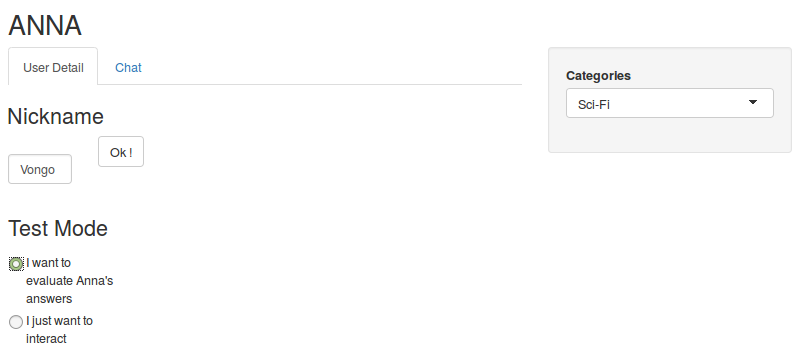
\includegraphics[width=0.70\textwidth]{./img/AnnaLoginUI.png}
\end{center}
\caption{LogIn Interface, where you can also decide whether you want to evaluate Anna's answers.}
\label{fig:AnnaLoginUI}
\end{figure}

\begin{figure}[!h]
\begin{center}
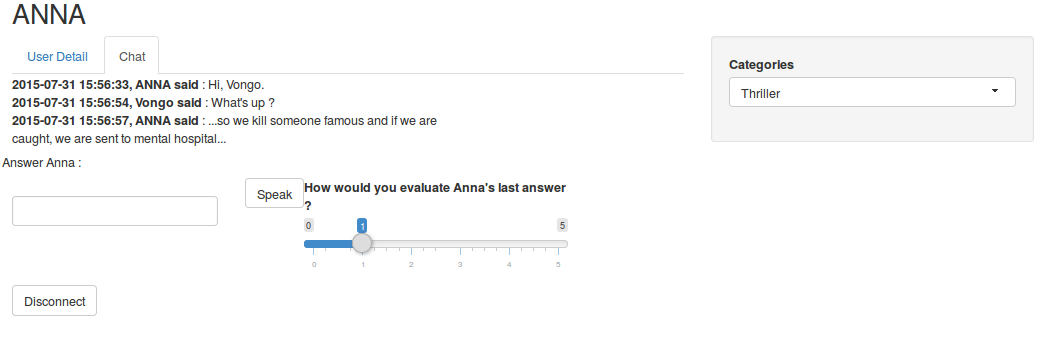
\includegraphics[width=0.80\textwidth]{./img/AnnaChatUI.png}
\end{center}
\caption{Chat Interface : a simple chat session.}
\label{fig:AnnaChatUI}
\end{figure}

\subsection{Architecture}
\label{sub:Architecture}


%
\subsection{Anna's answers}
\subsubsection{Version 1 : Random answers}
\label{sssec:v_rand}

\subsubsection{Version 2 : Determined SentenceType}
\label{sssec:v_stype}

\subsubsection{Version 3 : Determined movie genre}
\label{sssec:v_genre}
